% ============================================================
%  Beamer Presentation — Multimodal Sentiment Analysis
%  Team: TokeNization | Course: Introduction to NLP (S26)
%  Compile: pdflatex presentation.tex  (twice for ToC)
% ============================================================
\documentclass[aspectratio=169]{beamer}

\usetheme{Madrid}
\usecolortheme{default}

% Custom colours — a calm navy + orange accent palette
\definecolor{navyblue}{RGB}{25, 55, 109}
\definecolor{skyblue}{RGB}{173, 210, 240}
\definecolor{accentorange}{RGB}{220, 110, 30}
\definecolor{lightgray}{RGB}{245, 245, 245}
\definecolor{darkgray}{RGB}{80, 80, 80}
\definecolor{goodgreen}{RGB}{30, 140, 60}
\definecolor{warnred}{RGB}{180, 30, 30}

\setbeamercolor{palette primary}{bg=navyblue, fg=white}
\setbeamercolor{palette secondary}{bg=navyblue!85, fg=white}
\setbeamercolor{palette tertiary}{bg=navyblue!70, fg=white}
\setbeamercolor{palette quaternary}{bg=navyblue, fg=white}
\setbeamercolor{structure}{fg=navyblue}
\setbeamercolor{frametitle}{bg=navyblue, fg=white}
\setbeamercolor{title}{fg=white}
\setbeamercolor{block title}{bg=navyblue!90, fg=white}
\setbeamercolor{block body}{bg=navyblue!8}
\setbeamercolor{block title alerted}{bg=accentorange, fg=white}
\setbeamercolor{block body alerted}{bg=accentorange!12}
\setbeamercolor{block title example}{bg=goodgreen!80, fg=white}
\setbeamercolor{block body example}{bg=goodgreen!8}

% Fonts
\usepackage[T1]{fontenc}
\usepackage[utf8]{inputenc}
\usepackage{lmodern}
\usepackage{microtype}

% For tables
\usepackage{booktabs}
\usepackage{multirow}
\usepackage{array}
\usepackage{colortbl}

% For code-like text
\usepackage{listings}
\lstset{basicstyle=\tiny\ttfamily, backgroundcolor=\color{lightgray},
        frame=single, framesep=2pt, framexleftmargin=2pt, xleftmargin=4pt,
        breaklines=true, keywordstyle=\color{navyblue}\bfseries}

% For math / symbols
\usepackage{amsmath, amssymb}

% Tikz for simple diagrams
\usepackage{tikz}
\usetikzlibrary{positioning, arrows.meta, shapes.geometric, fit, backgrounds}

% Misc
\usepackage{graphicx}
\usepackage{hyperref}

% Remove navigation bar clutter
\setbeamertemplate{navigation symbols}{}

% Footline with page numbers
\setbeamertemplate{footline}{%
  \leavevmode%
  \hbox{\begin{beamercolorbox}[wd=.33\paperwidth,ht=2.25ex,dp=1ex,center]{palette secondary}%
    \usebeamerfont{author in head/foot}\insertshortauthor
  \end{beamercolorbox}%
  \begin{beamercolorbox}[wd=.34\paperwidth,ht=2.25ex,dp=1ex,center]{palette tertiary}%
    \usebeamerfont{title in head/foot}\insertshorttitle
  \end{beamercolorbox}%
  \begin{beamercolorbox}[wd=.33\paperwidth,ht=2.25ex,dp=1ex,right]{palette primary}%
    \usebeamerfont{author in head/foot}\insertframenumber{} / \inserttotalframenumber\hspace*{2ex}
  \end{beamercolorbox}}%
  \vskip0pt%
}

% ---- Title info ----
\title[Multimodal Sentiment Analysis]{Multimodal Sentiment Analysis\\via Multi-Layer Feature Fusion \& Multi-Task Learning}
\subtitle{A Re-implementation and Extension of Cai et al.\ (2025)}
\author[TokeNization]{Gautam Gandhi \and Manas Inamdar \and Parth Tokekar \and Soham Jahagirdar}
\institute[IIIT Hyderabad]{Introduction to NLP (S26) --- IIIT Hyderabad\\[4pt] \textbf{Team: TokeNization}}
\date{March 2026}

% ============================================================
\begin{document}

% ============================================================
%  TITLE SLIDE
% ============================================================
\begin{frame}[plain]
  \titlepage
\end{frame}

% ============================================================
%  OUTLINE
% ============================================================
\begin{frame}{What We'll Cover}
  \tableofcontents[hideallsubsections]
\end{frame}

% ============================================================
\section{The Paper \& The Problem}
% ============================================================

\begin{frame}{The Paper We're Implementing}
  \begin{columns}[T]
    \column{0.72\textwidth}
      \begin{block}{Reference}
        Cai et al., ``\textit{Multimodal sentiment analysis based on multi-layer feature
        fusion and multi-task learning},''\\
        \textbf{Scientific Reports} (2025), 15:2126.
      \end{block}

      \vspace{6pt}
      \textbf{Core idea in one sentence:}\\[4pt]
      Use \textbf{text + audio + video} together to predict how positive or negative
      someone feels — fusing all three using attention, trained with multiple
      simultaneous tasks.

      \vspace{8pt}
      \textbf{Key claim:} Better fusion + multi-task training gives\\
      \quad MAE = 0.728 \quad Acc-2 = 86.6\% \quad on CMU-MOSI.

    \column{0.28\textwidth}
      \begin{alertblock}{Our Goal}
        \small
        Re-implement this architecture from scratch in PyTorch and understand
        every design choice.
      \end{alertblock}
      \vspace{6pt}
      \begin{exampleblock}{Dataset}
        \small
        \textbf{CMU-MOSI}\\
        2,199 video clips\\
        sentiment: $-3$ to $+3$\\
        1,283 train / 214 val / 686 test
      \end{exampleblock}
  \end{columns}
\end{frame}

\begin{frame}{The Problem: Why is This Hard?}
  \begin{columns}[T]
    \column{0.48\textwidth}
      \textbf{What is Multimodal Sentiment Analysis?}
      \begin{itemize}
        \item Given a video clip of someone speaking, predict their sentiment score
        \item Use \textbf{text} (what they say), \textbf{audio} (how they say it),
          and \textbf{video} (what their face shows)
      \end{itemize}

      \vspace{6pt}
      \textbf{Why not just use text?}\\[3pt]
      In ``I \textit{absolutely loved} it'' with a \textit{flat voice} and
      \textit{blank face} — the words say positive but the person means the opposite.
      Text alone gets fooled by sarcasm and irony.

    \column{0.48\textwidth}
      \begin{alertblock}{Three Core Challenges}
        \begin{enumerate}
          \item \textbf{Different data types:} Text is 768-dim word vectors;
            audio is 74 acoustic measurements; video is 47 facial action scores.
            They live in very different spaces.
          \item \textbf{Conflicting signals:} One modality might say positive
            while another says negative. Which do you trust?
          \item \textbf{Text dominates:} Text alone gives $\sim$73\% accuracy.
            Audio and video add only a little — but they help on the hard cases.
        \end{enumerate}
      \end{alertblock}
  \end{columns}
\end{frame}

% ============================================================
\section{Architecture: What the Paper Proposes}
% ============================================================

\begin{frame}{Overall Architecture: Two Stages}
  \vspace{-4pt}
  \begin{center}
  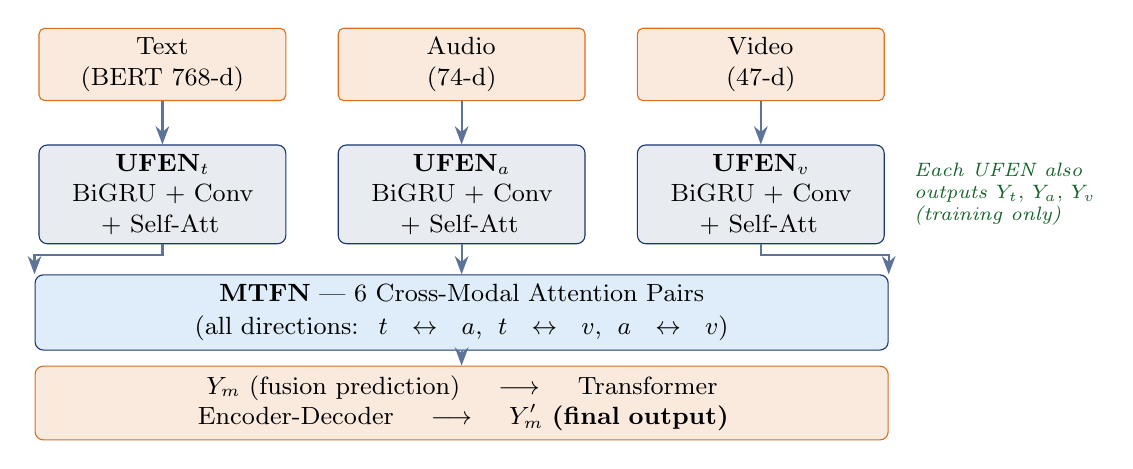
\begin{tikzpicture}[
    box/.style={draw=navyblue, fill=navyblue!10, rounded corners=3pt,
                minimum height=1.05cm, text width=2.9cm, align=center, font=\small},
    widebox/.style={draw=navyblue, fill=skyblue!40, rounded corners=3pt,
                minimum height=0.85cm, text width=10.6cm, align=center, font=\small},
    inp/.style={draw=accentorange, fill=accentorange!15, rounded corners=2pt,
                minimum height=0.65cm, text width=2.9cm, align=center, font=\small},
    arr/.style={-Stealth, thick, color=navyblue!70},
  ]
    %% Fixed x-positions: 0, 3.8, 7.6  (centred at 3.8)
    \node[inp] (xt) at (0,   0) {Text\\(BERT 768-d)};
    \node[inp] (xa) at (3.8, 0) {Audio\\(74-d)};
    \node[inp] (xv) at (7.6, 0) {Video\\(47-d)};

    \node[box] (ut) at (0,   -1.65) {\textbf{UFEN}$_t$\\BiGRU + Conv\\+ Self-Att};
    \node[box] (ua) at (3.8, -1.65) {\textbf{UFEN}$_a$\\BiGRU + Conv\\+ Self-Att};
    \node[box] (uv) at (7.6, -1.65) {\textbf{UFEN}$_v$\\BiGRU + Conv\\+ Self-Att};

    % Side note for unimodal heads
    \node[font=\scriptsize, text=goodgreen!70!black, align=left,
          right=0.25cm of uv] (ylbl)
      {\textit{Each UFEN also}\\
       \textit{outputs} $Y_t$, $Y_a$, $Y_v$\\
       \textit{(training only)}};

    \node[widebox] (mtfn) at (3.8, -3.15)
      {\textbf{MTFN} \textemdash{} 6 Cross-Modal Attention Pairs\\[1pt]
       (all directions:\; $t\!\leftrightarrow\!a$,\;
                         $t\!\leftrightarrow\!v$,\;
                         $a\!\leftrightarrow\!v$)};

    \node[widebox, fill=accentorange!15, draw=accentorange] (enc) at (3.8, -4.3)
      {$Y_m$ (fusion prediction) $\;\longrightarrow\;$
       Transformer Encoder-Decoder $\;\longrightarrow\;$
       $Y'_m$ \textbf{(final output)}};

    \draw[arr] (xt)--(ut);
    \draw[arr] (xa)--(ua);
    \draw[arr] (xv)--(uv);
    \draw[arr] (ut.south) -- ++(0,-0.14) -| (mtfn.north west);
    \draw[arr] (ua.south) -- (mtfn.north);
    \draw[arr] (uv.south) -- ++(0,-0.14) -| (mtfn.north east);
    \draw[arr] (mtfn)--(enc);
  \end{tikzpicture}
  \end{center}
  \vspace{2pt}
  \small
  \textbf{Stage 1 (UFEN):} Extract good features from each modality independently.\quad
  \textbf{Stage 2 (MTFN):} Combine all three modalities using attention.
\end{frame}

\begin{frame}{Complete System Pipeline (v2)}
  \vspace{-2pt}
  \begin{center}
    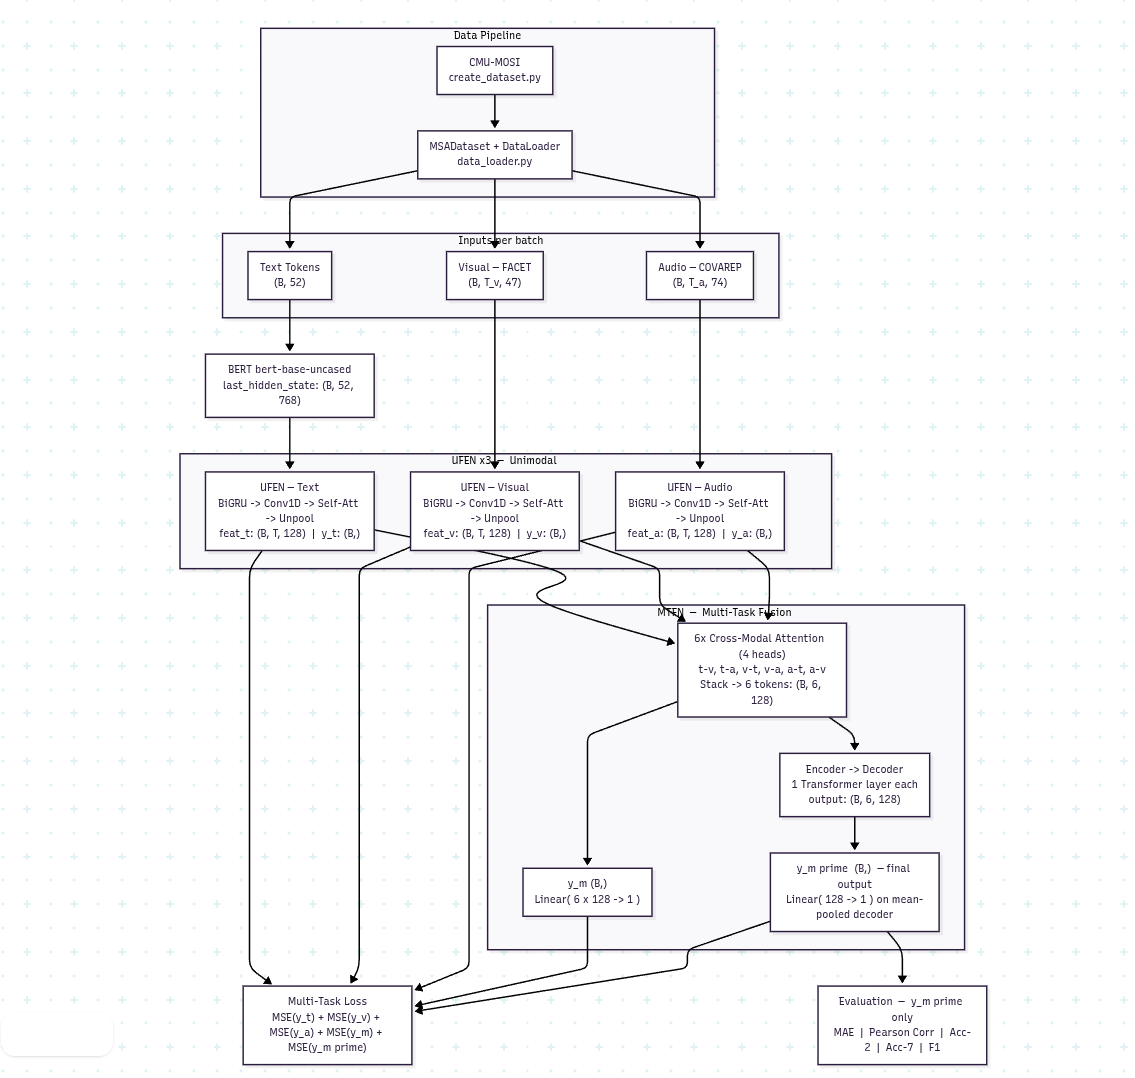
\includegraphics[width=0.60\textwidth, height=0.84\textheight, keepaspectratio]{images/img3.png}
  \end{center}
\end{frame}

\begin{frame}{Stage 1 — UFEN: Learning Features per Modality}
  \textbf{Why do we need UFEN?} Raw input features are noisy and have no temporal
  context understood by the network yet. UFEN builds a compact, context-aware
  representation for each modality.

  \bigskip

  \begin{columns}[T]
    \column{0.52\textwidth}
      \textbf{UFEN Pipeline (same structure for all 3 modalities):}
      \begin{enumerate}
        \item \textbf{Bi-GRU} — reads the sequence forward \emph{and} backward
          to capture context (e.g., ``not bad at all'' — the word ``bad'' gets
          corrected by what comes after it)
        \item \textbf{N parallel Conv1D branches} — detect local patterns of
          different widths (e.g., 1-word vs.\ 5-word windows)
        \item \textbf{Self-Attention gate} — let each time step decide how
          much other time steps matter for it; gates the conv output
        \item \textbf{Sum across branches} — combine multi-scale features
        \item \textbf{Unimodal prediction head} ($Y_t$, $Y_a$, $Y_v$) — used
          only during training
      \end{enumerate}

    \column{0.44\textwidth}
      \begin{block}{Why Bi-GRU?}
        \small A regular GRU only sees past words. Bidirectional also sees
        future words, which helps with word-order-sensitive sentiment.
      \end{block}
      \vspace{6pt}
      \begin{block}{Why Conv branches?}
        \small Short utterances (5--14 words average) benefit from local
        pattern detection at multiple scales — a single kernel misses either
        local or wider context.
      \end{block}
      \vspace{6pt}
      \begin{block}{Why self-attention gate?}
        \small Some time steps are more important than others. Self-attention
        assigns weights automatically — no manual feature selection.
      \end{block}
  \end{columns}
\end{frame}

\begin{frame}{UFEN: Forward Pass in Detail}
  \vspace{-2pt}
  \begin{center}
    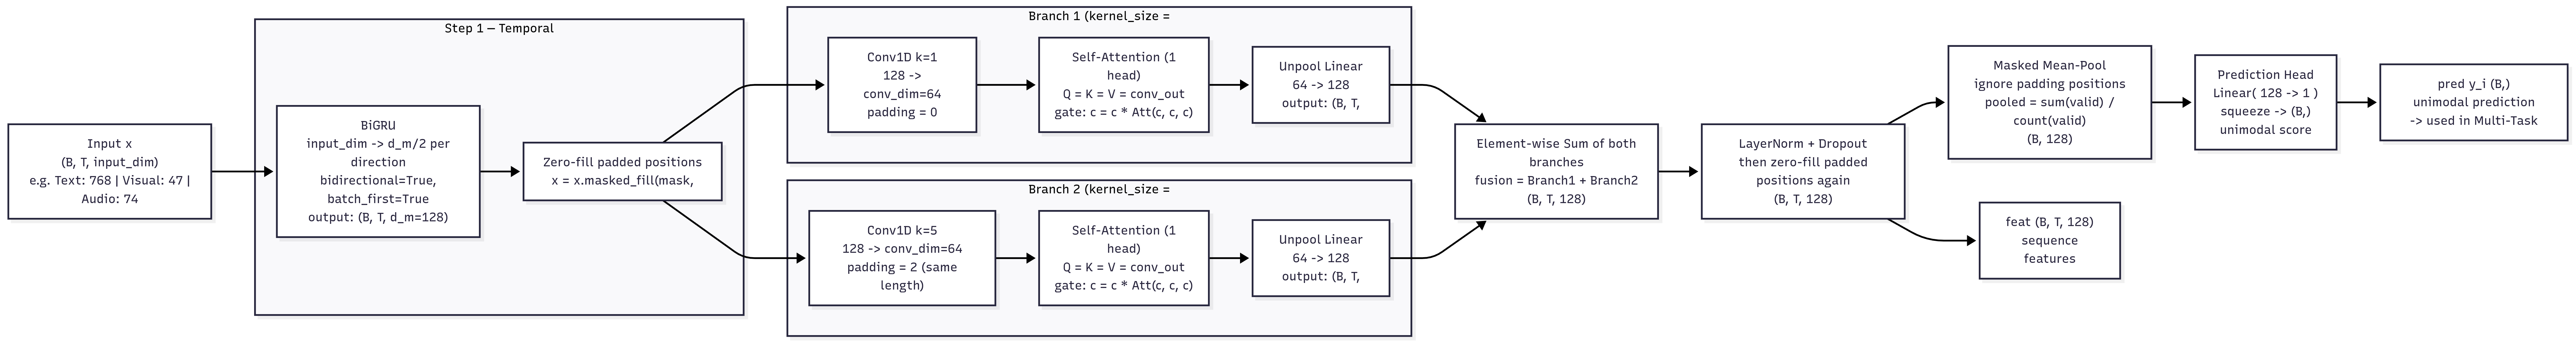
\includegraphics[width=\textwidth, height=0.84\textheight, keepaspectratio]{images/img2.png}
  \end{center}
\end{frame}

\begin{frame}{Stage 2 — MTFN: Fusing the Three Modalities}
  \vspace{-4pt}
  \begin{columns}[T]
    \column{0.50\textwidth}
      \small\textbf{Cross-Modal Attention (6 directed pairs):}

      \smallskip
      Each pair lets one modality \emph{ask questions} about another:
      \begin{itemize}\setlength{\itemsep}{1pt}
        \item Text asks: \emph{what does the audio confirm/contradict?}
        \item Audio asks: \emph{what emotion does the face confirm?}
        \item All 6 directions: $t\!\to\!a$, $t\!\to\!v$, $a\!\to\!t$,
              $a\!\to\!v$, $v\!\to\!t$, $v\!\to\!a$
      \end{itemize}

      \smallskip
      \textbf{Why cross-attention and not just concatenation?}\\
      Concatenation treats all features equally. Attention
      \emph{selectively} pulls in only the relevant parts of the other
      modality — crucial when modalities conflict.

    \column{0.46\textwidth}
      \small\textbf{Transformer Encoder-Decoder:}
      \begin{itemize}\setlength{\itemsep}{1pt}
        \item The 6 attention outputs are mean-pooled $\rightarrow$ 6 tokens
        \item Encoder: refines the 6 tokens using self-attention
        \item Decoder: produces the final representation $\rightarrow$ $Y'_m$
      \end{itemize}

      \vspace{4pt}
      \begin{alertblock}{Multi-Task Learning (5 losses!)}
        \small Loss = $\lambda_m \mathcal{L}_{m'} + \lambda_f \mathcal{L}_m
        + \lambda_t \mathcal{L}_t + \lambda_a \mathcal{L}_a
        + \lambda_v \mathcal{L}_v$

        \smallskip
        Training on all 5 heads forces each UFEN to stay useful on its own —
        prevents the model from ignoring audio/video.
      \end{alertblock}
  \end{columns}
\end{frame}

\begin{frame}{MTFN: Forward Pass in Detail}
  \vspace{-2pt}
  \begin{center}
    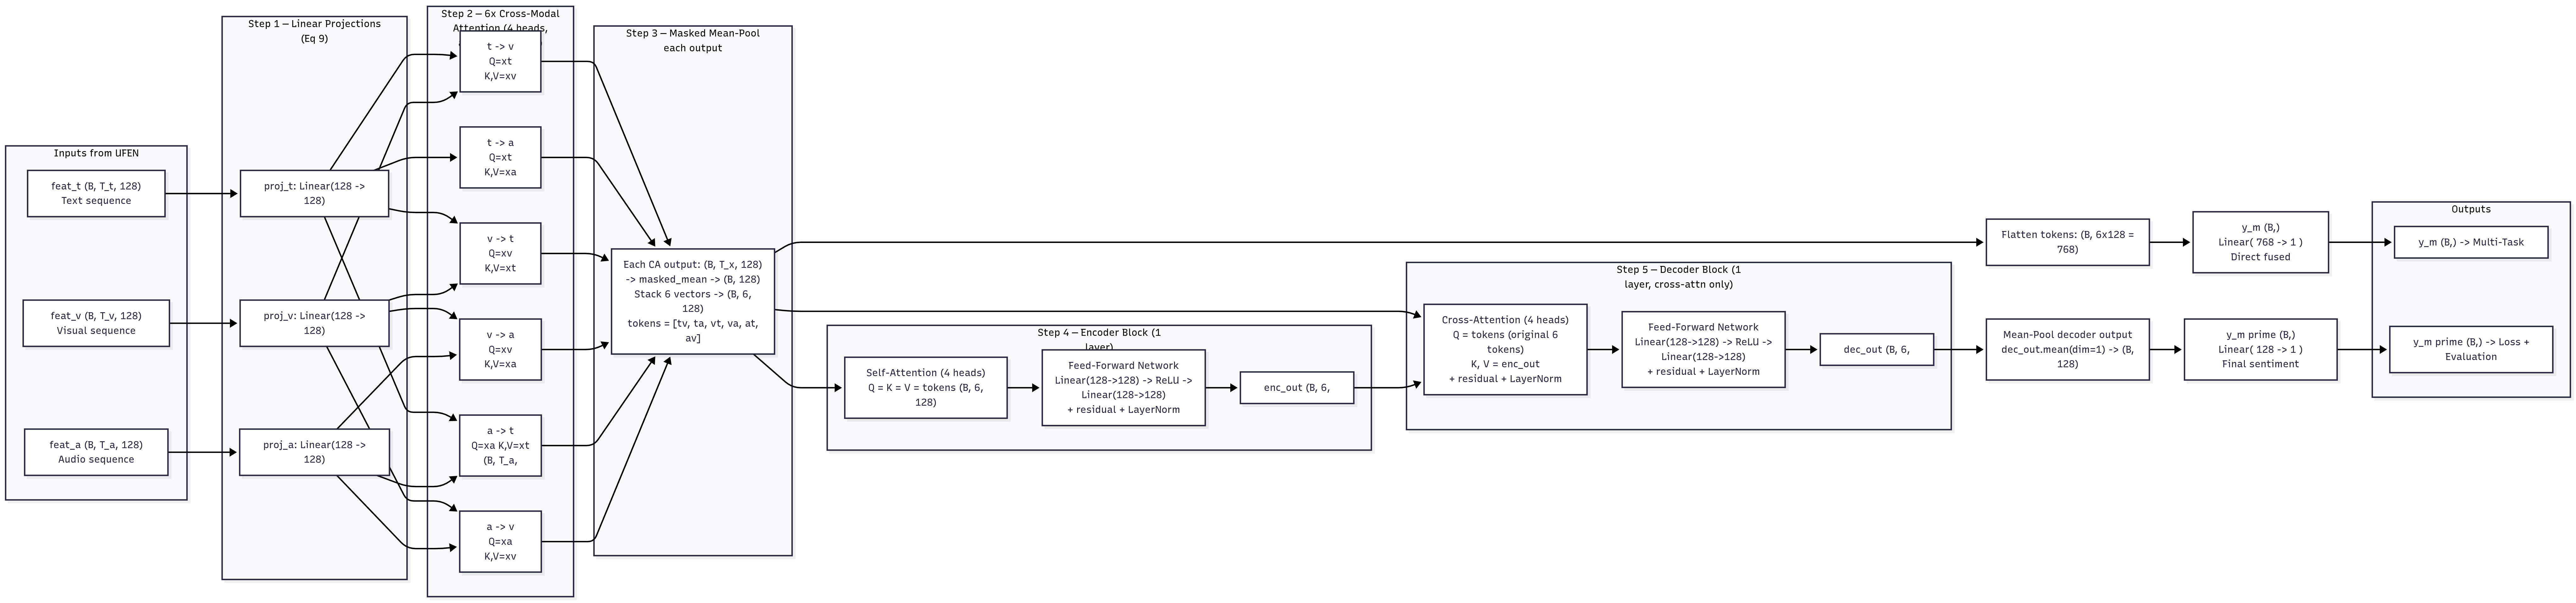
\includegraphics[width=\textwidth, height=0.84\textheight, keepaspectratio]{images/img1.png}
  \end{center}
\end{frame}

% ============================================================
\section{What the Paper Specifies vs. Our Assumptions}
% ============================================================

\begin{frame}{What the Paper Specifies Clearly}
  \vspace{-4pt}
  \begin{columns}[T]
    \column{0.50\textwidth}
      \small\textbf{Directly from Table 2 or the ablation study:}

      \smallskip
      \renewcommand{\arraystretch}{1.15}
      \begin{tabular}{lll}
        \toprule
        \textbf{Parameter} & \textbf{Value} & \textbf{Source} \\
        \midrule
        Self-att heads      & 1      & Table 2 \\
        Cross-att heads     & 4      & Table 2 \\
        Att dropout         & 0.2    & Table 2 \\
        Dropout             & 0.1    & Table 2 \\
        Starting LR         & 5e-3   & Table 2 \\
        Batch size          & 32     & Table 2 \\
        Epochs              & 30     & Table 2 \\
        Conv branches ($N$) & 2      & Ablation \\
        \bottomrule
      \end{tabular}

    \column{0.46\textwidth}
      \begin{alertblock}{What is \emph{not} specified}
        \small\begin{itemize}\setlength{\itemsep}{0pt}
          \item Hidden dimension $d_m$
          \item Conv kernel sizes
          \item Conv filter count
          \item FFN size in encoder-decoder
          \item Whether BERT is \textbf{frozen} or \textbf{fine-tuned}
          \item How to handle variable-length sequences
          \item LR to use for BERT
          \item Whether to use an LR schedule
        \end{itemize}
      \end{alertblock}
      \small These gaps forced us to make design decisions — and they turned
      out to be the most important decisions in the whole project.
  \end{columns}
\end{frame}

\begin{frame}{Our Key Assumptions}
  \vspace{-4pt}
  \begin{columns}[T]
    \column{0.50\textwidth}

    \begin{block}{Assumption 1 — BERT's Role}
      \footnotesize
      Paper calls it ``feature extractor'' (Experiments) but UFEN is described
      uniformly for all modalities (Methods). \textbf{Ambiguous:} frozen or fine-tuned?
    \end{block}

    \vspace{3pt}

    \begin{block}{Assumption 2 — $d_m = 128$}
      \footnotesize With 4 cross-attention heads, $d_m=128$ gives 32 dims/head —
      a standard choice. Never stated explicitly in the paper.
    \end{block}

    \vspace{3pt}

    \begin{block}{Assumption 3 — Conv kernels}
      \footnotesize
      Two parallel branches with different kernels: $k=1$ (per-word) and
      $k=5$ (local context), since utterances average 5--14 words.
    \end{block}

    \column{0.46\textwidth}

    \begin{block}{Assumption 4 — Softmax $\to$ Linear output}
      \footnotesize
      Paper writes $Y = \text{softmax}(Wx+b)$, but labels are continuous
      ($-3$ to $+3$). We use \texttt{Linear(d,1)} — softmax would break regression.
    \end{block}

    \vspace{3pt}

    \begin{block}{Assumption 5 — BERT LR separation}
      \footnotesize
      Paper says LR = 5e-3. Fine-tuning BERT at 5e-3 destroys pre-trained
      weights. Solution: BERT at 2e-5, rest at 5e-3.
    \end{block}

    \vspace{3pt}

    \begin{block}{Assumption 6 — Mean-pooling for fusion}
      \footnotesize
      Cross-attention outputs have variable length. We mean-pool each output
      over time $\to$ one vector per pair $\to$ stack to 6 tokens.
    \end{block}

  \end{columns}
\end{frame}

% ============================================================
\section{Phase 1: First Implementation}
% ============================================================

\begin{frame}{Phase 1 — First Implementation (\texttt{main} branch)}
  \vspace{-4pt}
  \small\textbf{A careful, conservative reading of the paper}

  \smallskip

  \begin{columns}[T]
    \column{0.50\textwidth}
      \small\textbf{Key design choices:}
      \begin{itemize}\setlength{\itemsep}{1pt}
        \item \textbf{BERT frozen} — text features pre-extracted once and saved
        \item \textbf{Sequential conv branches} — each layer feeds the next
          (kernel $= 3$ for all)
        \item \textbf{Shared cross-attention weights} — all 6 pairs share
          Q/K/V per modality (literal read of Eq.\ 9)
        \item Fixed $T = 30$; no padding masks
        \item Single LR = 5e-3 for all parameters
        \item Early stop patience = 8 on validation loss
      \end{itemize}

    \column{0.46\textwidth}
      \begin{block}{Architecture snapshot}
        \small
        \begin{tabular}{ll}
          $d_m$          & 64  \\
          $d_e$ (cross-att) & 64 \\
          GRU hidden     & 32 / direction \\
          Visual dim     & 35 (FACET 4.2) \\
          Total params   & \textbf{442,501} \\
        \end{tabular}
      \end{block}

      \vspace{4pt}
      \begin{alertblock}{Results}
        \small
        \begin{tabular}{ll}
          MAE $\downarrow$    & 0.981 \\
          Pearson Corr $\uparrow$ & 0.618 \\
          Acc-7 $\uparrow$   & 34.3\% \\
          Acc-2 (neg/pos) $\uparrow$ & 77.7\% \\
        \end{tabular}\\[2pt]
        \textit{Paper target: MAE 0.728, Acc-2 86.6\%}
      \end{alertblock}

      \vspace{3pt}
      \small
      Submitted as the \textbf{mid-semester report}.
  \end{columns}
\end{frame}

\begin{frame}{Why Phase 1's Numbers Were Lower}
  \vspace{-2pt}
  \begin{columns}[T]
    \column{0.48\textwidth}
      \small After the mid-submission we investigated \emph{why} the gap existed.

      \smallskip
      \textbf{Root cause analysis:}
      \begin{itemize}\setlength{\itemsep}{2pt}
        \item Frozen BERT: model \textbf{cannot adapt text representations}
          — static features, even for ambiguous sentiment words
        \item Early stop patience = 8 with noisy val-loss stopped
          training too early
        \item Single LR = 5e-3 with no schedule $\Rightarrow$ noisy convergence
        \item Zero-padding without masks pollutes attention and mean-pool
      \end{itemize}

    \column{0.48\textwidth}
      \begin{alertblock}{The biggest insight}
        \small
        Frozen BERT $\Rightarrow$ only \textbf{442K trainable parameters}
        from 1,283 training examples.\\[4pt]
        BERT representations are fixed — the model cannot learn that
        ``sick'' means \textit{great} in slang, or ``fine'' in a flat
        voice means \textit{unhappy}.\\[4pt]
        \textbf{Fine-tuning BERT is likely what the paper intended},
        despite the ``feature extractor'' wording.
      \end{alertblock}
  \end{columns}
\end{frame}

% ============================================================
\section{Phase 2: Improved Architecture (v2)}
% ============================================================

\begin{frame}{After More Research — What We Changed for v2}
  \vspace{-4pt}
  \small\textbf{After the mid-submission, we continued experimenting and built
  a revised implementation (\texttt{ufen-mtfn-v2}).}

  \smallskip

  \renewcommand{\arraystretch}{1.12}
  \small
  \begin{tabular}{p{3.6cm} p{3.8cm} p{3.8cm}}
    \toprule
    \textbf{Dimension} & \textbf{Phase 1 (main)} & \textbf{Phase 2 (v2)} \\
    \midrule
    BERT               & Frozen, pre-extracted   & \cellcolor{goodgreen!20}Fine-tuned live \\
    Total parameters   & 442K                    & \cellcolor{goodgreen!20}110.8M \\
    Conv branches      & Sequential, same kernel & \cellcolor{goodgreen!20}Parallel, $k=1$ and $k=5$ \\
    Cross-attention    & Shared Q/K/V (6 pairs)  & \cellcolor{goodgreen!20}6 independent modules \\
    Padding masks      & Not used                & \cellcolor{goodgreen!20}Full mask propagation \\
    LR strategy        & Single 5e-3             & \cellcolor{goodgreen!20}Dual: 5e-3 + 2e-5 (BERT) \\
    LR schedule        & None                    & \cellcolor{goodgreen!20}Cosine + BERT warmup \\
    $d_m$              & 64                      & \cellcolor{goodgreen!20}128 \\
    Visual dim         & 35                      & \cellcolor{goodgreen!20}47 \\
    \bottomrule
  \end{tabular}
\end{frame}

\begin{frame}{Key Difference 1 — BERT: Frozen vs.\ Fine-tuned}
  \vspace{-4pt}
  \begin{columns}[T]
    \column{0.50\textwidth}
      \small\textbf{Phase 1 (frozen BERT):}
      \begin{itemize}\setlength{\itemsep}{1pt}
        \item BERT runs once, saves 768-dim vectors to disk
        \item Vectors never change during training
        \item Model learns on top of fixed representations
        \item Only 442K parameters are trainable
      \end{itemize}

      \vspace{4pt}
      \small\textbf{Phase 2 (fine-tuned BERT):}
      \begin{itemize}\setlength{\itemsep}{1pt}
        \item BERT runs inside every forward pass
        \item Weights update at small LR (2e-5) to preserve pre-trained knowledge
        \item Text representations adapt continuously to predict sentiment
        \item 110M parameters become trainable
      \end{itemize}

    \column{0.46\textwidth}
      \begin{alertblock}{Why does fine-tuning help so much?}
        \small
        BERT is pre-trained on generic language. Sentiment has domain-specific
        patterns (sarcasm, hedging, intensifiers) the generic representations
        don't capture well.\\[4pt]
        Fine-tuning lets BERT specialise for sentiment on top of its
        broad knowledge.
      \end{alertblock}

      \vspace{4pt}
      \begin{exampleblock}{The BERT warmup trick}
        \small
        BERT is frozen for the first 5 epochs so the rest of the model
        stabilises, \emph{then} BERT is unfrozen. This prevents chaotic
        gradients from destroying BERT at startup.
      \end{exampleblock}
  \end{columns}
\end{frame}

\begin{frame}{Key Difference 2 — Conv Branches: Sequential vs.\ Parallel}
  \begin{columns}[T]
    \column{0.48\textwidth}
      \textbf{Phase 1 — Sequential:}

      \medskip
      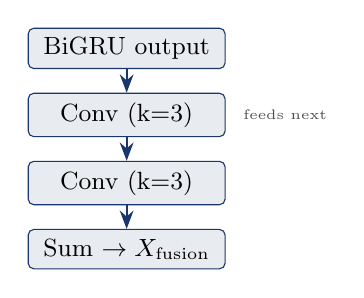
\begin{tikzpicture}[
        box/.style={draw=navyblue, fill=navyblue!10, minimum width=2.5cm,
                    minimum height=0.5cm, align=center, font=\small, rounded corners=2pt},
        arr/.style={-Stealth, thick, navyblue}
      ]
        \node[box] (b) {BiGRU output};
        \node[box, below=0.3cm of b] (c1) {Conv (k=3)};
        \node[box, below=0.3cm of c1] (c2) {Conv (k=3)};
        \node[box, below=0.3cm of c2] (s) {Sum $\to X_\text{fusion}$};
        \draw[arr] (b)--(c1);
        \draw[arr] (c1)--(c2);
        \draw[arr] (c2)--(s);
        \node[right=0.1cm of c1, font=\tiny, text=darkgray] {feeds next};
      \end{tikzpicture}

      \vspace{4pt}
      \small Each conv layer reads \emph{the previous layer's output}.
      Both branches use the same kernel size.

    \column{0.48\textwidth}
      \textbf{Phase 2 — Parallel:}

      \medskip
      \begin{tikzpicture}[
        box/.style={draw=navyblue, fill=navyblue!10, minimum width=2cm,
                    minimum height=0.5cm, align=center, font=\small, rounded corners=2pt},
        arr/.style={-Stealth, thick, navyblue}
      ]
        \node[box] (b) {BiGRU output};
        \coordinate (split) at ($(b.south)+(0,-0.3)$);
        \node[box, below left=0.4cm and 0.3cm of b] (c1) {Conv (k=1)};
        \node[box, below right=0.4cm and 0.3cm of b] (c2) {Conv (k=5)};
        \node[box, below=1.2cm of b] (s) {Sum $\to X_\text{fusion}$};
        \draw[arr] (b.south) -- ++(0,-0.15) -| (c1.north);
        \draw[arr] (b.south) -- ++(0,-0.15) -| (c2.north);
        \draw[arr] (c1.south) |- (s.west);
        \draw[arr] (c2.south) |- (s.east);
        \node[below=0.05cm of c1, font=\tiny, text=darkgray] {pointwise};
        \node[below=0.05cm of c2, font=\tiny, text=darkgray] {5-word window};
      \end{tikzpicture}

      \vspace{4pt}
      \small Both branches read the \emph{same} BiGRU output.
      Different kernels give multi-scale features.
  \end{columns}
  \vspace{4pt}
  \small
  \textbf{Why parallel is better:} The paper says ``$N$ \emph{parallel} branches'' —
  parallel directly matches that wording. Different kernel sizes let the model
  capture both per-word features ($k=1$) and short-phrase features ($k=5$) simultaneously.
\end{frame}

\begin{frame}{Key Difference 3 — Training Strategy}
  \begin{columns}[T]
    \column{0.50\textwidth}
      \textbf{Phase 1 — Simple training:}
      \begin{itemize}
        \item Single LR = 5e-3 for \emph{all} parameters
        \item No learning rate schedule
        \item Early stop on total validation loss\\
          (sum of 5 sub-task MSE losses)
        \item Patience = 8 epochs
      \end{itemize}

      \vspace{6pt}
      \textbf{Problem:} Validation total loss is dominated by the 3 unimodal
      sub-tasks. The model can stop early even if the main combined output
      is still improving.

    \column{0.46\textwidth}
      \textbf{Phase 2 — Richer training:}
      \begin{itemize}
        \item \textbf{Dual learning rates:}
          \begin{itemize}
            \item 5e-3 for non-BERT parameters (fresh, needs to learn fast)
            \item 2e-5 for BERT (pre-trained, needs gentle updates)
          \end{itemize}
        \item \textbf{Cosine LR schedule} — smoothly decays LR over 50
          epochs instead of keeping it constant
        \item \textbf{BERT warmup} — BERT is frozen for 5 epochs, then
          unfrozen gradually
        \item Early stop on \textbf{dev MAE directly} — what we actually
          care about
        \item Patience = 15 epochs
      \end{itemize}
  \end{columns}
\end{frame}

% ============================================================
\section{Results \& Comparison}
% ============================================================

\begin{frame}{Results: Phase 1 vs Phase 2 vs Paper Target}
  \vspace{-2pt}
  \begin{center}
  \renewcommand{\arraystretch}{1.4}
  \begin{tabular}{lcccc}
    \toprule
    \textbf{Metric} &
    \textbf{Phase 1} &
    \textbf{Phase 2} &
    \textbf{Improvement} &
    \textbf{Paper Target} \\
    \midrule
    MAE $\downarrow$     & 0.981 & \textbf{0.812} &
      \cellcolor{goodgreen!20}$-$0.169 & 0.728 \\
    Pearson Corr $\uparrow$ & 0.618 & \textbf{0.745} &
      \cellcolor{goodgreen!20}$+$0.127 & 0.792 \\
    Acc-7 $\uparrow$     & 34.3\% & \textbf{43.0\%} &
      \cellcolor{goodgreen!20}$+$8.7pp & 46.7\% \\
    Acc-2 (neg/pos) $\uparrow$ & 77.7\% & \textbf{80.3\%} &
      \cellcolor{goodgreen!20}$+$2.6pp & 86.6\% \\
    \midrule
    Trainable params & 442K & 110.8M & --- & --- \\
    \bottomrule
  \end{tabular}
  \end{center}

  \vspace{6pt}
  \begin{columns}[T]
    \column{0.48\textwidth}
      \begin{exampleblock}{Best run (P3-2 config)}
        \small
        50 epochs total, early stopped at epoch 42\\
        Best dev MAE = 0.7434 (close to paper's 0.728)\\
        Test MAE = 0.812 — small dev/test gap of 0.069
      \end{exampleblock}
    \column{0.48\textwidth}
      \begin{alertblock}{What's still missing vs.\ paper}
        \small
        The remaining gap likely comes from: norm differences
        in their data preprocessing, exact FACET/COVAREP feature
        versions, and possible differences in multi-task loss weights.
      \end{alertblock}
  \end{columns}
\end{frame}

\begin{frame}{What Made the Biggest Difference}
  \vspace{-4pt}
  \begin{columns}[T]
    \column{0.50\textwidth}
      \small We ran 25+ experiments across 3 phases to isolate each factor:

      \smallskip
      \renewcommand{\arraystretch}{1.15}
      \small
      \begin{tabular}{lll}
        \toprule
        \textbf{Change} & \textbf{MAE gain} & \textbf{Impact} \\
        \midrule
        BERT fine-tuning  & $\sim -0.12$ & \cellcolor{goodgreen!30}Very high \\
        Cosine LR + warmup & $\sim -0.03$ & \cellcolor{goodgreen!15}Medium \\
        Parallel conv + larger $k$ & $\sim -0.02$ & \cellcolor{goodgreen!10}Moderate \\
        Masked mean-pool  & $\sim -0.01$ & Minor \\
        Early stop on MAE & $\sim -0.01$ & Minor \\
        \bottomrule
      \end{tabular}

    \column{0.46\textwidth}
      \begin{alertblock}{Key lesson}
        \small
        Whether to freeze or fine-tune BERT accounts for
        \textbf{the majority of the gap} between Phase 1 and Phase 2.\\[4pt]
        Many papers say ``BERT as feature extractor'' but actually
        fine-tune it in code. We had to determine the right interpretation
        experimentally.
      \end{alertblock}

      \vspace{4pt}
      \begin{block}{Also important}
        \small
        Proper LR scheduling and metric-targeted early stopping had a
        clear effect on final numbers.
      \end{block}
  \end{columns}
\end{frame}

% ============================================================
\section{Verdict \& Next Steps}
% ============================================================

\begin{frame}{Which Design Choices Were Right?}
  \vspace{-4pt}
  \renewcommand{\arraystretch}{1.12}
  \small
  \begin{tabular}{p{3.2cm}p{3.0cm}p{3.0cm}p{2.4cm}}
    \toprule
    \textbf{Decision} & \textbf{Phase 1} & \textbf{Phase 2} & \textbf{Verdict} \\
    \midrule
    BERT role    & Frozen & Fine-tuned &
      \cellcolor{goodgreen!20}v2 correct \\
    Conv design  & Sequential, $k=3$ & Parallel, $k\!=\!1, 5$ &
      \cellcolor{goodgreen!20}v2 closer \\
    Cross-att weights & Shared & Independent &
      Both defensible \\
    Padding masks & Not used & Full masking &
      \cellcolor{goodgreen!20}v2 rigorous \\
    Early stop metric & Total val loss & Dev MAE &
      \cellcolor{goodgreen!20}v2 better \\
    LR schedule  & None & Cosine + warmup &
      \cellcolor{goodgreen!20}Clearly helpful \\
    Z-score norm & Applied & Not applied &
      Phase 1 better \\
    \bottomrule
  \end{tabular}

  \vspace{4pt}
  \small
  Phase 1's Z-score normalisation is \textbf{the one thing Phase 1 did better} —
  cleaning extreme COVAREP artifact values ($\approx -3.4 \times 10^{38}$) that
  v2 skips, relying on model adaptation instead.
\end{frame}

\begin{frame}{Next Steps}
  \begin{columns}[T]
    \column{0.50\textwidth}
      \textbf{Near-term experiments on CMU-MOSI:}
      \begin{itemize}
        \item Try LR = 2e-3 for non-BERT params to reduce the learning rate
          asymmetry (current: 250:1 ratio, BERT vs.\ non-BERT)
        \item Add Z-score normalisation from Phase 1 into v2 preprocessing
        \item Explore SWA (Stochastic Weight Averaging) — a technique that
          averages model weights over the last few epochs to improve
          generalisation; already implemented in Phase 1's code
      \end{itemize}

    \column{0.46\textwidth}
      \textbf{Project Phase 2 — MELD dataset:}
      \begin{itemize}
        \item Adapt the UFEN+MTFN architecture for \textbf{emotion
          classification} (7 classes: Anger, Disgust, Sadness, Joy,
          Neutral, Surprise, Fear)
        \item Replace regression head with softmax classification
        \item Training objective: Cross-Entropy instead of MSE
        \item Evaluate with weighted F1 (class imbalance in MELD)
        \item Qualitative analysis: visualise attention weights on
          sarcastic clips to see if model uses facial cues correctly
      \end{itemize}
  \end{columns}
\end{frame}

% ============================================================
\section{Summary}
% ============================================================

\begin{frame}{Summary}
  \begin{columns}[T]
    \column{0.50\textwidth}
      \textbf{What we implemented:}
      \begin{itemize}
        \item Full PyTorch re-implementation of UFEN + MTFN from
          Cai et al.\ (2025)\\
        \item Two versions with careful documentation of every design
          choice and assumption\\
        \item 25+ systematic experiments across 3 phases to understand
          what matters most
      \end{itemize}

      \vspace{8pt}
      \textbf{Best result achieved (Phase 2):}
      \medskip
      \begin{tabular}{ll}
        MAE             & \textbf{0.812} (paper: 0.728) \\
        Pearson Corr    & \textbf{0.745} (paper: 0.792) \\
        Acc-2           & \textbf{80.3\%} (paper: 86.6\%) \\
        Acc-7           & \textbf{43.0\%} (paper: 46.7\%) \\
      \end{tabular}

    \column{0.46\textwidth}
      \begin{block}{Key takeaways}
        \begin{enumerate}
          \item \textbf{BERT fine-tuning is the most important decision} —
            ambiguous paper wording led to Phase 1 keeping BERT frozen,
            which was the root cause of the large performance gap.
          \item \textbf{Architecture details matter} — parallel convolutions
            with multi-scale kernels outperform sequential same-kernel branches.
          \item \textbf{Training setup matters} — proper LR scheduling and
            metric-targeted early stopping are often as important as the
            architecture itself.
        \end{enumerate}
      \end{block}

      \vspace{4pt}
      \small
      Code: \url{https://github.com/Gautam-Gandhi/Multimodal-Sentiment-Analysis}\\
      Branch: \texttt{ufen-mtfn-v2}
  \end{columns}
\end{frame}

% ============================================================
%  THANK YOU
% ============================================================
\begin{frame}[plain]
  \vfill
  \begin{center}
    {\Large\color{navyblue}\textbf{Thank You!}}

    \vspace{16pt}
    \begin{tabular}{cc}
      Gautam Gandhi & Manas Inamdar \\[4pt]
      Parth Tokekar & Soham Jahagirdar \\
    \end{tabular}

    \vspace{14pt}
    \textit{Introduction to NLP (S26) — Team TokeNization}\\[6pt]
    \footnotesize
    Cai et al.\ (2025). ``Multimodal sentiment analysis based on multi-layer
    feature fusion and multi-task learning.'' \textit{Scientific Reports}, 15:2126.
  \end{center}
  \vfill
\end{frame}

\end{document}
